\subsection{Passivity Analysis}
The stability analysis of the system gives information about the stability region of the proposed controller. We analyze passivity by observing the evolution of the kinetic energy of the system, given as:
\begin{equation}
	W(\vecs \xi, \vecs{\dot \xi}) = \frac{1}{2}  \dot{\vecs{\xi}}^T \matd{M}(\vecs \xi) \dot{\vecs{\xi}} \label{eq:energy_system}
\end{equation}

\begin{lemma} \label{lemma:passivity}
  % Let $\vect f(\vecs \xi)$ be the desired velocity with bounded magnitude, i.e., $\| \vect f(\xi) \| < \infty, \forall \xi \in \mathbb{R}^N$.
   Let us assume a robotic system as described in \eqref{eq:robot_dynamics} is controlled using \eqref{eq:control_command} using the damping matrix $\matd D(\vecs \xi)$ given in \eqref{eq:damping_summation} with damping values $s_d = 1, d = 1 .. N$.
   The system is passive with respect to the input-output pair $\vecs \xi_e$, $\vecs{\dot \xi}$ when exceeding the desired velocity $\vect f(\vecs \xi)$ , i.e., $\dot{W} \leq \vecs{\dot \xi}^T \vecs \tau^e, \; \forall \vecs \xi \in \mathbb{R}^N: \| \vecs{\dot \xi} \| \geq \| \vect f(\vecs \xi) \|$ and the storage function being the kinetic energy $W \in \mathbb{R}_{>0}$ given in \eqref{eq:energy_system}
\end{lemma}

\begin{proof}
The time derivative of storage function $W$ can be evaluated as:
\begin{align}
  % \begin{split}
	& \dot W(\vecs \xi, \vecs{\dot \xi}) =
    \vecs{\dot \xi}^T \matd M(\vecs \xi) \vecs{\ddot \xi}  + \frac{1}{2} \vecs{\dot \xi}^T \dot{\matd M}(\vecs \xi) \vecs{\dot \xi}  \nonumber \\
  &= \frac{1}{2} \vecs{\dot \xi}^T \left( \dot{\matd M}(\vecs \xi) - 2 \matd C(\vecs \xi) \right) \dot{\vecs \xi} - \vecs{\dot \xi}^T \matd{D}(\vecs \xi) \left(\vecs{\dot \xi} - \vect f(\vecs \xi) \right) + \vecs{\dot \xi}^T \vecs \tau^e \nonumber \\
  &= - \vecs{\dot \xi}^T \matd{D}(\vecs \xi) \left( \vecs{\dot\xi} - \mathbf{f}(\vecs \xi) \right) + \vecs{\dot\xi}^T \vecs{\tau}^e
  % \end{split}
\end{align}
where the second order dynamics $\vecs{\ddot \xi}$ are evaluated according to the rigid body dynamics defined in \eqref{eq:robot_dynamics}. Furthermore, $\dot{\matd M} - 2 \matd C$ is skew-symmetric for any physical system; hence, the corresponding summand is zero.

% \subsubsection{Stability with Uniform Damping}
Let us investigate the region where the passivity holds. Since in the Lemma, we assumed all damping values to be equal to one, we have:
\begin{equation}
	\matd{D}({\vecs \xi}) = \matd{Q}({\vecs \xi}) \matd{S} ({\vecs \xi}) \matd{Q}({\vecs \xi})^{-1}= \matd{Q}({\vecs \xi}) \matd{I} \matd{Q}({\vecs \xi})^{-1} = \matd{I}
\end{equation}
where $\matd{I} \in \mathbb{R}^{N \times N}$ is the identity matrix.

It follows that the system is passive with respect to the input, the external force $\tau^e$, and the output, the velocity $\dot {\vecs \xi}$, if: 
\begin{equation}
	\dot{\boldsymbol {\vecs \xi}}^T \matd{D}({\vecs \xi}) \left(\dot{\boldsymbol {\vecs \xi}} - \boldsymbol{f}(\boldsymbol {\vecs \xi}) \right) = 
    \dot{{\vecs \xi}} ^ T \Delta \vect{f}  \geq 0 
 \; , \quad
 \Delta \vect{f} = \dot{{\vecs \xi}} - \vect{f}({\vecs \xi})
 \label{eq:passivity_condition}
\end{equation}

On the border of this region, the two vectors $\Delta \vect{f}$ and $\dot{{\vecs \xi}}$ are orthogonal.
Hence, using Thale's theorem, this region can be interpreted as a circle in velocity-space with radius $\| \vect{f} ({\vecs \xi}) \| / 2$ and center $\vect{f}({\vecs \xi}) / 2$, see Figure~\ref{fig:passivity_analysis}.

\begin{figure}[bh]
	\centering
	% \includesvg[width=0.7\columnwidth]{figures/passivity_analysis.svg}
	\ifthesis
    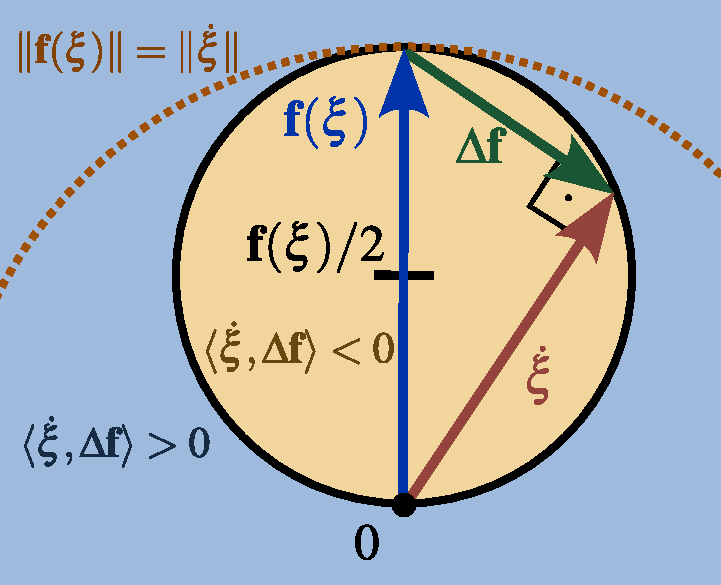
\includegraphics[width=0.7\columnwidth]{figures/passivity_analysis}
	\else
    % 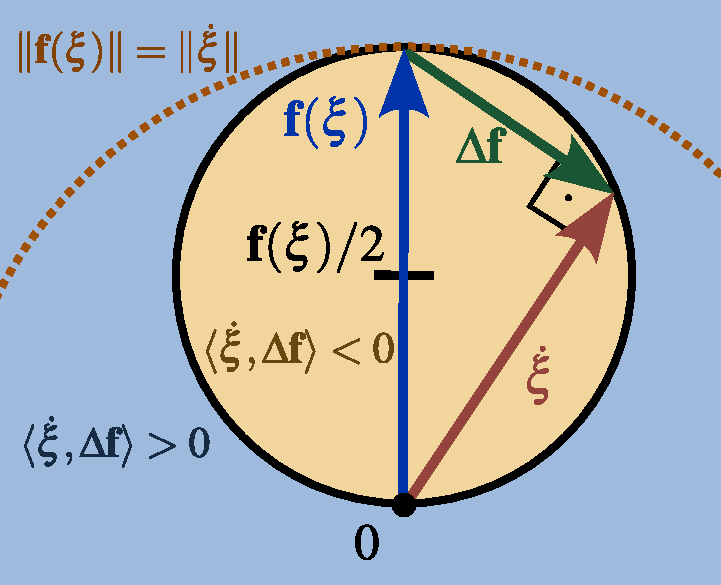
\includegraphics[width=.8\columnwidth]{figures/passivity_analysis}
    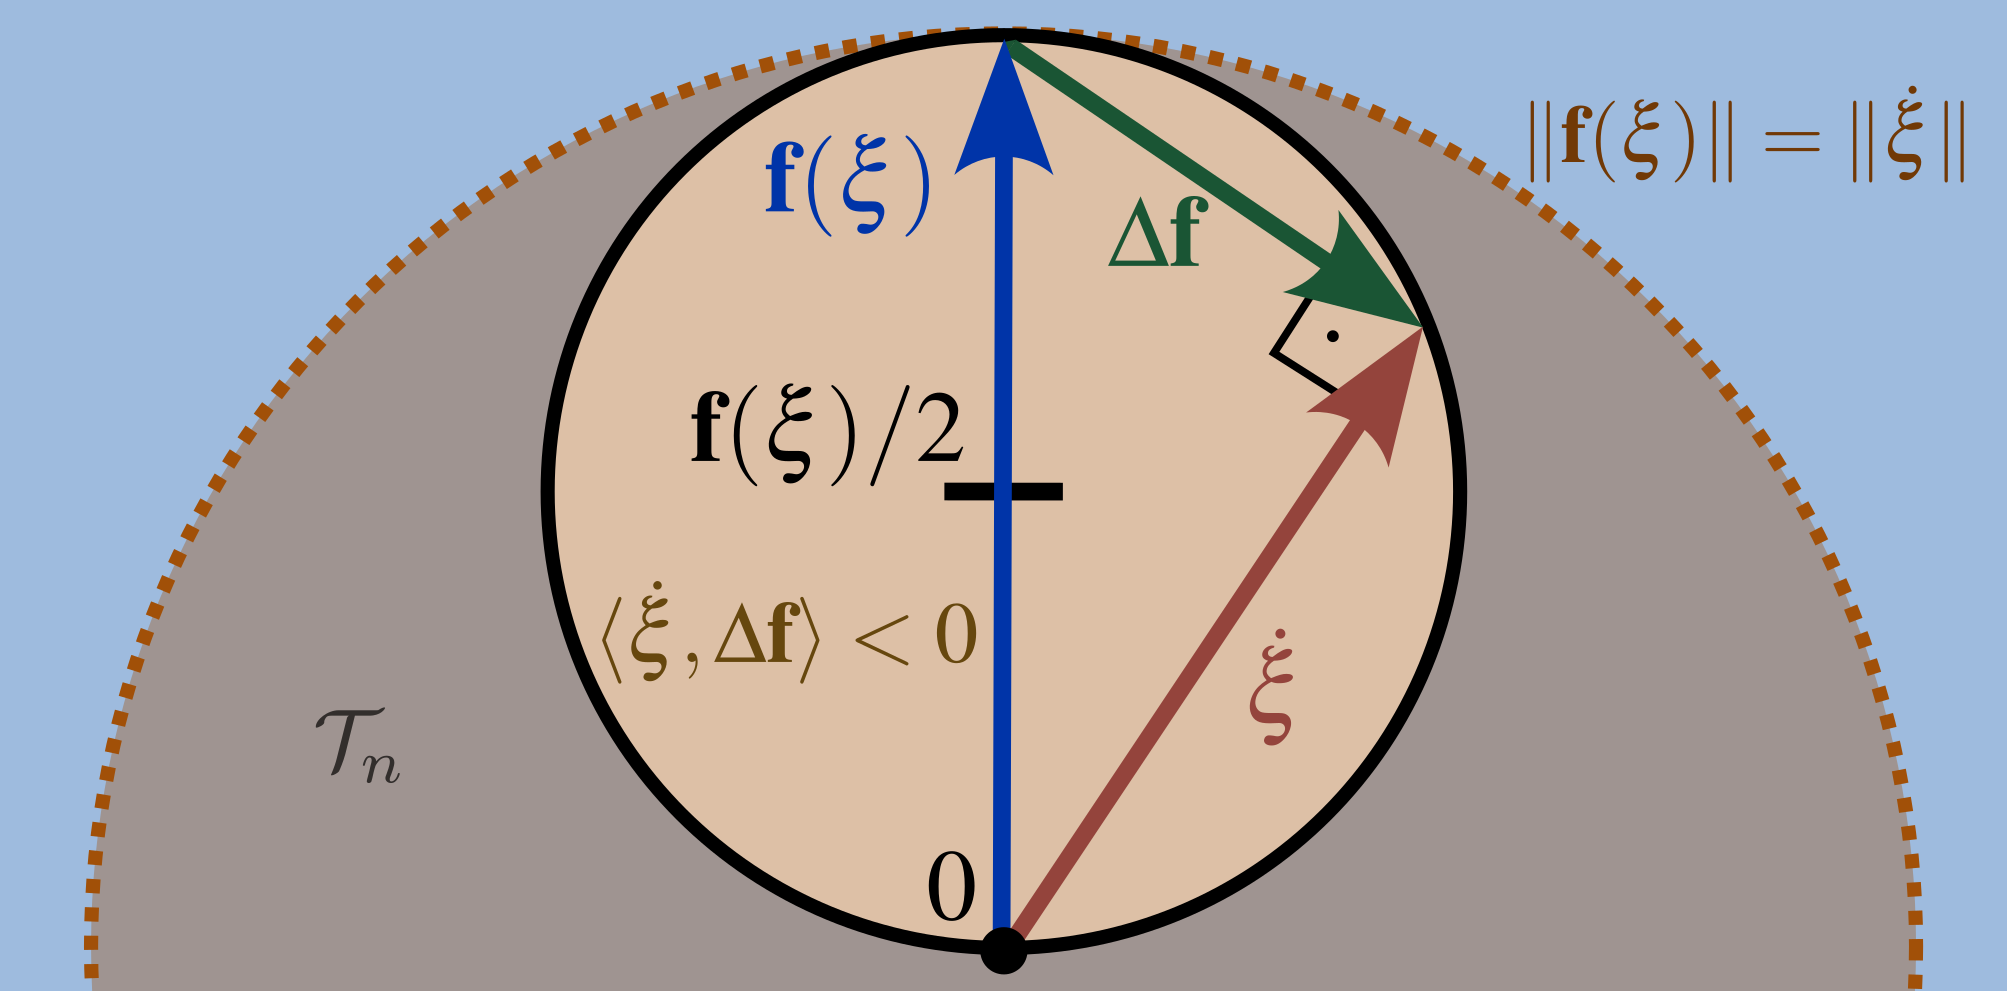
\includegraphics[width=.8\columnwidth]{figures/passivity_analysis.png}
	\fi
	\caption{Analyzing the system in velocity-space yields that the system is passive if it has a velocity $\dot{\vecs \xi}$ larger than the desired velocity $\vect f(\vecs \xi)$, i.e., outside the dashed circle.
    However, the system can be non-passive for small velocities when  $\dotprod{\dot{\vecs \xi}}{\Delta \vect f} < 0$ (yellow circle).}
	\label{fig:passivity_analysis}
\end{figure}

Moreover, the system is passive as long as the observed velocity $\dot{{\vecs \xi}}$ is outside the circular-red region, which is a subset of the region where the magnitude of the observed velocity is smaller than the desired velocity $\vect {f}({\vecs \xi})$, i.e.,
\begin{equation}
	\dot W({\vecs \xi}, \dot{{\vecs \xi}}) \leq \dot{{\vecs \xi}}^T \vecs \tau^e
 \quad \forall {\vecs \xi} : \| \dot{{\vecs \xi}} \| \geq\| \vect{f}({\vecs \xi}) \| 
\end{equation}

\end{proof}

As in the orange region, the system is not passive; the storage function $W$ could increase, and hence, the velocity $\dot {\vecs \xi}$ increases non-passively. This behavior is not unexpected, as the controller is designed to approach the desired dynamics $\vect{f}({\vecs \xi})$. Hence, as long as the desired velocity is not reached, the kinetic energy increases even with no force input $\vecs \tau^e$. However, as soon as the system velocity $\dot{\vecs \xi}$ exceeds the desired velocity $\vect f(\vecs \xi)$, the system behaves passively. We can use this to ensure the stability of the system:

\begin{theorem}  \label{theorem:passivity}
  Let $\vect f(\vecs \xi)$ is the desired velocity with bounded magnitude, i.e., $\| \vect f(\vecs \xi) \| < v^{\mathrm{max}}, \forall \vecs \xi \in \mathbb{R}^N$.
   The closed loop system \eqref{eq:robot_dynamics} using the controller from \eqref{eq:control_command} and the damping matrix $\matd D(\vecs \xi)$ given in \eqref{eq:damping_summation} is bounded-input, bounded-output (BIBO) stable with respect to the input disturbance force $\vect \tau^e$, and output the velocity $\dot{\vecs \xi}$ for all times $T = 0, \, .., \, \infty$.
\end{theorem}
 
\begin{proof}
% From Lemma~\ref{lemma:passivity}, the system is passive when the magnitude of the velocity is larger than the dynamics, i.e. $\| \dot{\vecs \xi} \| > \|\vect f(\vecs \xi) \|$, the orange circle in Figure~\ref{fig:passivity_analysis}.
% The system is not passive inside this region, and the velocity $\dot {\vecs \xi}$ can increase. However, the velocity increase is limited to staying below $\| \vect f({\vecs \xi}) \|$ before the system enters the region where it is passive. Hence, the control cannot introduce unexpected energy.
% It follows that the system has a bounded output as long as the desired velocity $\vecs{f}({\vecs \xi})$ is stable and the input $\int_{0}^T \dot{{\vecs \xi}}^T \vecs \tau^e dt$ is bounded. 

To ensure BIBO stability, let us analyze the integral of the impulse of the response for the external force $\vecs \tau^e$: 
\begin{equation}
	\begin{split}
	  \int_{0}^{T} \left\| \dot{\vecs \xi} \right\| \; dt 
	  & = \int_{t \notin \mathcal{T}_n} \left\| \dot {\vecs \xi} \right\|  \, dt + \int_{t \in  \mathcal{T}_n} \left\| \dot {\vecs \xi} \right\| \;  dt \\ 
	  % & = \int_{t : \| \dot{\vecs \xi} \| > \| \vect f(\vecs \xi) \|} \dot {\vecs \xi} \, dt + \int_{t : \| \dot{\vecs \xi} \| \leq \| \vect f(\vecs \xi) \|} \dot {\vecs \xi} \;  dt \\ 
	  % & \leq \int_{t \notin \mathcal{T}_n} \left| \dot {\vecs \xi} \right| dt + v^{\mathrm{max}}  T_n \\ 
	  & \leq K_p + v^{\mathrm{max}} T_n
\end{split}
\label{eq:bibo_velocity}
\end{equation}
where $\mathcal{T}_n$ denotes the set of time instances where the system is not shown to be passive (Fig.~\ref{fig:passivity_analysis}), specifically $\| \dot{\vecs \xi} \| \leq \| \vecs f (\vecs \xi) \|$, and $T_n \in \mathbb{R}_{\geq 0}$ is the total duration which the system spends in this region. Additionally, from passivity in the inner region, the system is bounded by a constant $K_p \in \mathbb{R}_{\geq 0}$.
Hence, the impulse response is bounded, and the system is BIBO stable.

% \subsubsection{Stability with General Damping}
However, from \eqref{eq:damping_summation}, we know that a general damping matrix $\matd{S}(\vecs \xi)$ can have non-uniform diagonal values. This is analyzed by introducing the coordinate transfers:
\begin{equation}
	\vecs{\bar{v}} = \sqrt{\matd{S}({\vecs \xi})} \matd{Q}({\vecs \xi})^{-1} \dot{{\vecs \xi}}
	\;\; \text{and} \;\;
	\bar{\Delta \vect f} = \sqrt{\matd{S}({\vecs \xi})} \matd{Q}({\vecs \xi})^{-1} \Delta \vect{f}
\end{equation}
where the square root of the diagonal matrix $\matd{S}({\vecs \xi})$ is taken element-wise.
The transfer is then used to rewrite \eqref{eq:passivity_condition} as:
\begin{equation}
\dot{\vecs \xi}^T \matd{D}({\vecs \xi}) \Delta \vect{f} = \vecs{\dot \xi}^T \matd{Q}({\vecs \xi}) \matd{S}({\vecs \xi}) \matd{Q}({\vecs \xi})^{-1} \Delta \vect{f} = \vecs{\bar v}^T \bar{\Delta \vect f}
\end{equation}

Hence, the BIBO analysis of \eqref{eq:bibo_velocity} applied to the transformed system results as:
\begin{equation}
\begin{split}
	  & \int_{0}^{T} \left\| \vecs{\bar v} \right\| \; dt   
	   = \int_{t \notin \bar{\mathcal{T}}_n} \left\| \vecs{\bar v} \right\|  \, dt + \int_{t \in  \bar{\mathcal{T}}_n} \left\| \vecs{\bar v} \right\| \;  dt  \\ 
   & < K_p + v^{\mathrm{max}} \bar T_n 
   {\max{\Bigl(\text{eig}\bigl(\mathcal{D} \bigr) \Bigr)}} 
   / {\min{\Bigl(\text{eig}\bigl(\mathcal{D} \bigr) \Bigr)}}
\end{split}
\end{equation}
where $\bar{\mathcal{T}}_n$ denotes the region where the transformed system $\vecs{\bar v}$ is not shown to be passive, i.e. $\| \vecs{\bar v} \| \leq \| \bar{\Delta \vect f} \|$, and $\bar T_n \in \mathbb{R}_{\geq 0}$ the corresponding time. Additionally, $\min{(\text{eig}(\mathcal{D}))}$ and $\max{(\text{eig}(\mathcal{D}))}$ are the smallest and largest eigenvalue of the damping matrix $\matd{D}$ respectively.

Hence, since the transformed system with velocity $\vect {\bar v}$ is BIBO stable, the original system with velocity $\dot{\vecs \xi}$ is BIBO stable, too, as long as it is a continuous, finite transform. 
\end{proof}
% The analysis described in Fig.~\ref{fig:passivity_analysis} can hence be applied in the transformed space, too. 

For an orthogonal decomposition matrix $\matd{Q}(\boldsymbol{{\vecs \xi}})$, the region of non-passivity is an ellipse where the direction of the axes points along column vectors of $\matd{Q}({\vecs \xi})$, and the corresponding axes lengths are the diagonal elements of $\| \mathbf{f}({\vecs \xi})^T \sqrt{\matd{S}({\vecs \xi})}\| / 2 \sqrt{\matd{S}({\vecs \xi})}^{(-1)}$. 
If the ratio of the first damping value to the other axis $i \geq 2$ is large, i.e., $s_1 / s_i \gg 1$, it can lead to non-passivity even though the velocity $\dot{\vecs \xi}$ is already larger (but not pointing in the correct direction) than the desired velocity. However, the non-passive region is still \iflong bounded (Fig.\ref{fig:passivity_analysis_skew}). \else bounded. \fi
This proof holds for any basis $\matd{Q}$ which is not singular. However, the controller must be carefully chosen to ensure that the speed up is limited when the basis is close to singular, for example, by limiting the relative difference of the stretching vectors. Furthermore, as stable behavior is ensured for a general shape of a damping matrix $\matd{D}(\vecs \xi)$, the global stability proof extends to any positive definite damping matrix matrices.

Since the damping matrix $\matd D(\vecs \xi)$ changes dynamically, a change in the environment can move the system outside of the passive region. However, a finite maximum velocity always exists, at which the system is ensured to be passive.

\iflong
\begin{figure}[htbp]
    \centering
    \begin{subfigure}{0.49\columnwidth}
      \centerline{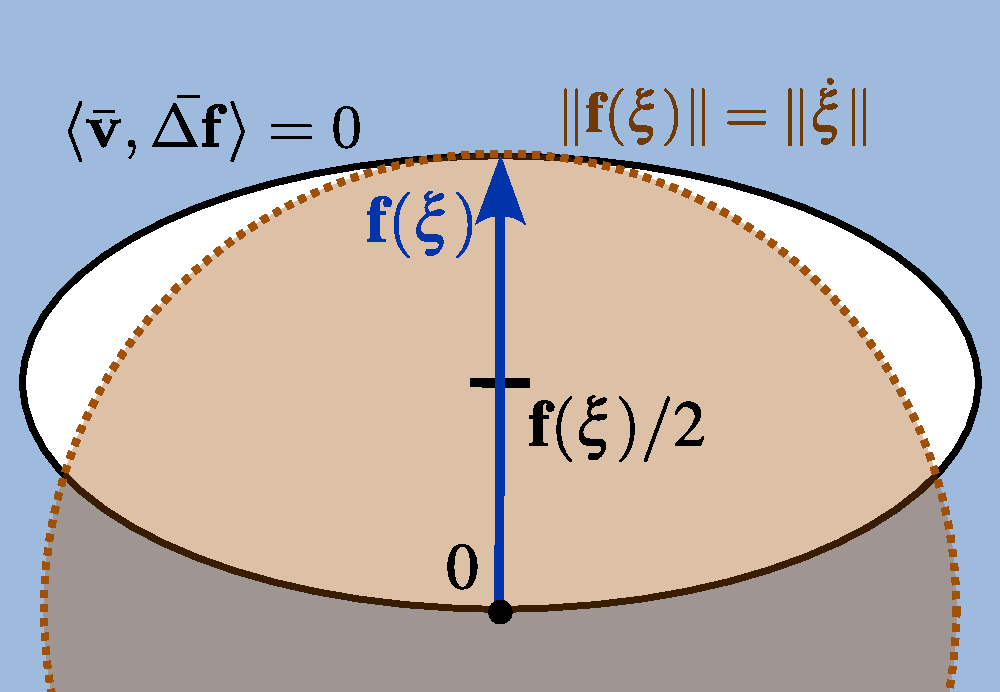
\includegraphics[width=\textwidth]{figures/passivity_analysis_wide}}
	  \caption{$\matd{S}_1^f > \matd{S}_2^f$, $w \approx 0$}
	  \label{fig:passivity_analysis_wide}
    \end{subfigure}\hfill%
    \begin{subfigure}{0.49\columnwidth}
    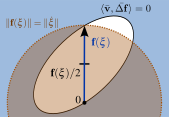
\includegraphics[width=\textwidth]{figures/passivity_analysis_skew}
	\caption{$\dotprod{\vect f(\vecs \xi)}{\vect q_1} \neq \| \vect f(\vecs \xi)\| \; \| \vect q_2\| $ }
      \label{fig:passivity_analysis_skew}
    \end{subfigure}
	\caption{
		The stability is ensured even if the controller can temporarily accelerate the system to reach a velocity $\dot{\vecs \xi}$, which is faster than the desired velocity $\vect f(\vecs \xi)$ (white region).
		This happens when the eigenvalues of the damping matrix $\matd{D}(\vecs \xi)$ are not uniform (a) or the stretching vectors $\vect q_1$ and $\vect q_2$ are not orthogonal (b). 
	In both cases, the region of non-passivity is elliptical (black circle).
}
	\label{fig:passivity_analysis_varied}
\end{figure}
\fi


% Note, that in the case of $\langle e_2, e_n \rangle \neq 0$ the choice of $e_2$ does not matter as the corresponding  weight from \eqref{eq:eig2_weight} is $w_2 = 0$, hence it $\lambda_2 = \lambda$, as all eigenvalues.
